  Das Internet hat sich in den letzten Jahren zu einem strategisch wichtigen
  Vertriebskanal entwickelt. Viele Unternehmen haben das erkannt und setzen im
  Betriebsalltag die Möglichkeiten ein, die das Internet als Vertriebskanal
  bietet. In der Finanzindustrie wurde dieser Schritt mit dem Online-Banking
  gegen Ende der Neunzigerjahre gemacht. Dabei wurden einige Dienstleistungen
  mit einer Web Applikation über das Internet nutzbar gemacht, die sonst beim
  klassischen Bankschalter bezogen werden konnten. Dass eine Onlinestrategie
  funktioniert und die Nachfrage dafür besteht, hat sich in den letzten Jahren
  in der Finanzindustrie gezeigt.
  
  Die Informatik spielt in der Finanzindustrie im Allgemeinen eine wichtige
  Rolle. Viele Finanzinstitute, hier in der Schweiz, zählen heute zu den
  grössten Arbeitgebern in der Informatik, siehe
  \cite{WoArbeitenInformatikfachleute}. Insgesammt gibt es in der Schweiz acht
  Unternehmen, welche selber nicht aus der Informatik Branche kommen, die mehr
  als 500 Informatikfachleute beschäftigen. Die Hälfte davon sind
  Finanzinstitute, namentlich sind das Credit Suisse, UBS, Zürich Versicherung
  und die Post. In der \ac{ZKB} ist die Informatik ebenfalls stark vertreten.
  
  Durch die zunehmende Komplexität im Finanzgeschäft, reicht manchmal 
  erwerbliche Softwarelösungen nicht vollends aus. Um den Vorsprung zur
  Konkurenz auszubauen, werden vielmals Computerprogramme in der
  Finanzindustrie selber entwickelt, welche die Automatisierung ihrer Prozesse
  ermöglicht oder mit denen Arbeiten in ihrem Kerngeschäft verrichtet werden
  können.
  
  Aus einer eigens entwickelten Lösung heraus kann sich ein neues Geschäft für
  das Finanzinstitut eröffnen. Eine solche Software könnte beispielsweise
  externen Vermögensverwaltern zur Verfügung gestellt werden. Dabei gibt es
  verschiedene Vertriebskanäle für Softwareprodukte. Das Internet ist einer
  davon. Er hat sich mit dem Onlinebanking bewährt und könnte sich somit auch
  für andere bestehende Lösungen eignen.
  
  In der \ac{ZKB} existieren viele solcher Lösungen bereits. Diese sind
  aber nicht für eine Online-Strategie entwickelt worden, sondern für den
  internen Einsatz. Einige dieser Programme wurden als Desktop Applikationen
  entwickelt, das entspricht den Anforderungen für den internen Einsatz. Um den
  Vertrieb zentral verwalten zu können, macht das Umrüsten bestehender Desktop
  Applikationen auf eine Online-Lösung Sinn.
  
  \section{Motivation}
  
  Die Zürcher Kantonalbank setzt bei der Entwicklung von Inhouse
  Softwarelösungen auf Java Swing Applikationen und auf Java Web Applikationen.
  Die Java Web Applikationen basieren auf dem Web Framework Apache Struts
  1.3.10 mit einer von der ZKB erstellten Erweiterung namens \ac{ZIP}. Da eine
  Lösung als Java Web Applikation zentral verwaltet werden kann, gibt es
  erhebliche Einsparungen im Bereich Testing, Deployment und Patching. Somit
  sollen in Zukunft Java Swing Applikationen auf Java Web Applikationen
  umgerüstet werden.
  
  Das Framework Apache Struts 1.3.10 ist mittlerweile in die Jahre gekommen. Es
  basiert auf dem Prinzip von ``full site reload''. Wann immer eine Aktion
  von einem User in der Applikation ausgeführt wird, sei es das Ansteuern eines
  Links oder das Absenden eines Formulars, wird die Webseite, welche die
  Applikation repräsentiert, vollständig neu geladen. Heutzutage gibt es
  Frameworks, welche einem ermöglichen eine Web Applikation zu entwickeln, die
  sich bei der Bedienung wie eine klassische Desktop Applikation anfühlt. Dabei
  werden nur Bereiche neu geladen, wo sich die zu darstellenden Informationen
  geändert haben. Dies wird durch die Technik von \ac{Ajax}\footnote{XML ist
  nicht zwingend, es kann auch mit JSON oder anderen Technologien gelöst
  werden.} realisiert.
  
  Bei \ac{Ajax} können Daten einer Web Applikation, ohne die komplette Webseite
  neu zu laden, verändert werden. Dies erlaubt es Web Applikationen, auf
  Benutzeraktionen schneller zu reagieren, da vermieden wird, dass statische
  Daten, die sich unter Umständen nicht verändert haben, immer wieder neu
  übertragen werden. Das beinhaltet nicht nur die sichtbaren Informationen,
  sondern auch die \ac{HTML}, \ac{CSS} und Java Script Ressourcen, die für die
  Darstellung notwendig sind.
  
  Apache Struts 1.3.10 unterstützt \ac{Ajax} nicht direkt, das kann über
  Erweiterungen ermöglicht werden. Es gibt Java Web Frameworks, welche diese
  Technik ``out of the box'' mitbringen. Eine Evaluation soll zeigen, ob eines
  dieser Java Web Frameworks besser für eine Anwendung geeignet ist.
  
  \section{Zielsetzung}
  
  Gegenstand der vorliegenden Diplomarbeit ist die Analyse, welche Java Web
  Frameworks für die Ablösung von bestehenden Java Swing Applikationen in Frage
  kommen. Es sollen anhand eines strukturierten Vorgehens eine Menge von
  bestehenden Java Swing Applikationen der Zürcher Kantonalbank auf deren
  Funktionalität der Benutzeroberfläche eruiert werden. Aufgrund der
  Anforderungen der IT-Architektur der Zürcher Kantonalbank sollen Java Web
  Frameworks auf die Validität der erhobenen Funktionalität verifiziert
  werden. Die Java Web Frameworks, welchen diesen Ansprüchen genügen, sollen
  auf einen möglichen Einsatz in der Informatik Infrastruktur der Züricher
  Kantonalbank untersucht werden. Durch die Implementierung eines Prototypen
  soll gezeigt werden, dass die Umsetzung möglich ist. Schlussendlich soll eine
  Empfehlung für ein Java Web Framework ausgesprochen werden, für den Fall,
  dass eine bestehende Java Swing Applikation in eine Web Applikation umgebaut
  werden soll. Ebenso sollen die gewonnen Erkenntnisse, für zukünftige
  Revisionen im Bereich der Java Web Frameworks der IT-Architektur der
  Zürcher Kantonalbank, als Grundlage dienen können.
  
  \section{Struktur}
  
  Die Arbeit wurde in sechs Teile gegliedert. Diese Teile bauen aufeinander auf
  und setzten meistens die Erkenntnisse der vorhergehenden Bestandteile voraus.
  
  \begin{description}
    
  \item[Einführung]
  
  Im Kapitel \ref{chapter:Einfuehrung} \nameref{chapter:Einfuehrung} wird die
  Motivation für die Diplomarbeit erläutert, ebenso wird auf die Zielsetzung
  eingegangen. Die Gliederung des Berichts wird in der Struktur
  aufgeschlüsselt. Im Ablauf wird gezeigt wie die Diplomarbeit durchgeführt
  wurde. Zudem befindet sich hier auch eine Danksagung.
  
  \item[Basisinformationen]
    
  In den Kapiteln 
  \ref{chapter:JavaSwingApplikationen} \nameref{chapter:JavaSwingApplikationen}
  und \ref{chapter:RichInternetApplikationen}
  \nameref{chapter:RichInternetApplikationen} werden Hintergrundinformationen
  zu diesen Themen vermittelt. Dabei werden hauptsächlich Begriffe aus diesen
  Bereichen erklärt und mit Hilfe von Abbildungen dargestellt. Die
  Informationen welche erläutert werden, dienen als Grundlage für die weiteren
  Kapitel und auch für das Verständnis des Themas.

  \item[Methoden]
  
  In den Kapiteln
  \ref{chapter:MethodenZurAnalyseVonJavaSwingApplikationen}
  \nameref{chapter:MethodenZurAnalyseVonJavaSwingApplikationen} und
  \ref{chapter:MethodenZurEntscheidungsfindungBeiEinerEvaluation}
  \nameref{chapter:MethodenZurEntscheidungsfindungBeiEinerEvaluation} werden
  Methoden erarbeitet. Diese Methoden sollen für die Durchführung, der in der
  Aufgabenstellung gestellten Aufgaben, verwendet werden.
  
  \item[Aufgaben]
  
  In den Kapiteln \ref{chapter:AnalyseDerInfrastrukturDerZuercherKantonalbank}
  bis \ref{chapter:ProofOfConcept} werden die erwarteten Ergebnisse
  entsprechend der Aufgabenstellung erarbeitet. Das beinhaltet die
  \nameref{chapter:AnalyseDerInfrastrukturDerZuercherKantonalbank} und die
  \nameref{chapter:AnalyseDerJavaSwingApplikationen}. Die
  \nameref{chapter:EvaluationDerJavaWebFrameworks} mit sinnvollen
  Rahmenbedingungen in der Form von Soll- und KO-Kriterien. Mit den erhaltenen
  Resultaten, wird die Integration in die ZKB Infrastruktur und die
  Implementierung der gefundenen Swingkomponenten geprüft. Als Abschluss werden
  im Kapitel \nameref{chapter:ProofOfConcept} die erarbeiteten Ergenisse bestätigt.
  
  \item[Erkenntnisse]
  
  Die Kapitel \ref{chapter:EmpfehlungFuerEinJavaWebFramework} und
  \ref{chapter:Reflexion} wiederspiegeln die Erkenntnisse, welche im Laufe
  der Diplomarbeit gewonnen wurden. Dabei wird eine
  \nameref{chapter:EmpfehlungFuerEinJavaWebFramework} für die Züricher
  Kantonalbank ausgepsrochen. Mit einer \nameref{chapter:Reflexion} sollen
  dargelegte theoretische Grundlagen, die gewählten Methoden sowie die
  Auswertung der Ergebnisse untersucht werden. Zudem wird ein Ausblick gewährt.
  
  \item[Anhang]
  
  Im Anhang sind Informationen zu finden, die entweder mit den
  \nameref{chapter:Rahmenbedingungen} der Diplomarbeit zu tun haben, wie das
  \nameref{chapter:Personalienblatt}, die \nameref{chapter:Aufgabenstellung}
  oder die Protokolle zu den offiziellen Terminen. Oder es handelt sich um
  Zusatzinformationen, welche vom Umfang her zu kostspielig gewesen sind, dass
  sie in der Arbeit Platz gefunden hätten, darunter fallen die
  \nameref{chapter:GrundsaetzeDerZkbItArchitektur} und die
  \nameref{chapter:18AnforderungenNachAgileLearn}. Ein spezieller Anhang
  beinhaltet die \nameref{chapter:Projektadministration}, in der die ganze
  Planung und Nachvollziehbarkeit der getätigten Aufgaben beschrieben wird.
  Zudem befinden sich hier auch sämtliche Verzeichnisse, insbesondere das
  \bibname.
  
  \end{description}
  
  \section{Ablauf}

  Der Ablauf der Kernaufgaben der Diplomarbeit wurde so strukturiert, dass die
  aufeinander folgenden Teile auf die jeweils vorher erarbeiteten Resultate
  aufbauen. Bilder sagen manachmal mehr als Worte, desshalb wurde der Ablauf in
  Form eines Flussdiagramms in der Abbildung
  \ref{img:durchfuehrungDerDiplomarbeit} dargestellt.
  
  Zusätzlich zu den dargestellten Aufgaben der Diplomarbeit kommen noch
  die Planung, Meetings, das Verfassen der Dokumentation und der Präsentationen,
  und vieles mehr. Diese Aspekte der Diplomarbeit sind in der Abbildung
  \ref{img:durchfuehrungDerDiplomarbeit} nicht ersichtlich.
  \newline
  
  \begin{figure}[htbp]
    \begin{center}
      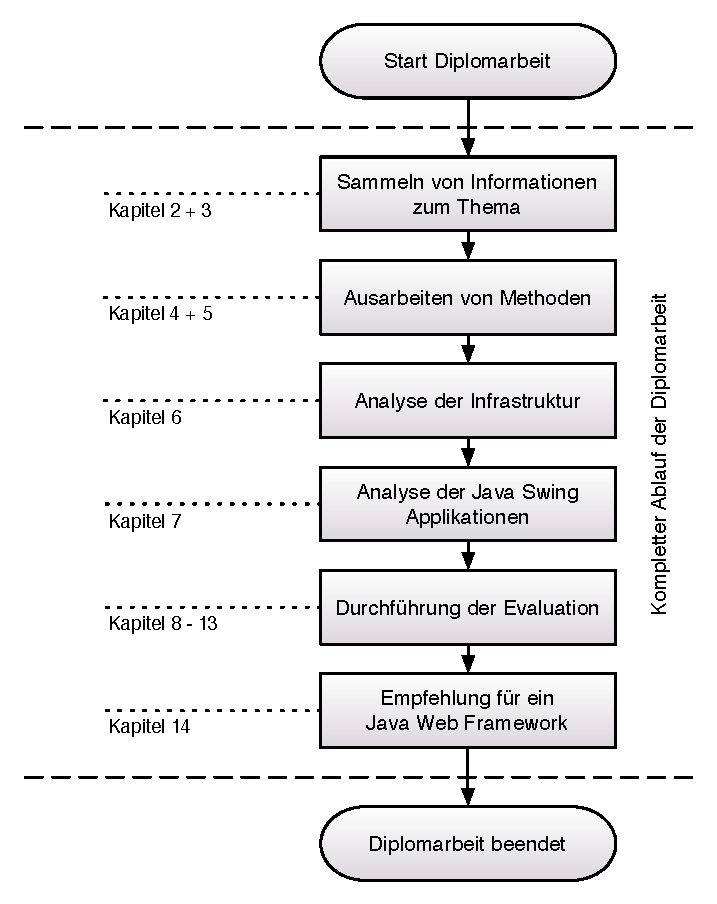
\includegraphics[width=0.65\textwidth]{./image/durchfuehrungDerDiplomarbeit.pdf}
      \caption{Strukturierte Durchführung der Diplomarbeit}
      \label{img:durchfuehrungDerDiplomarbeit}
    \end{center}
  \end{figure}
    